\chapter{Программная среда комплекс моделирования нелинейных динамических систем ``qontrol''}
\label{chapter_qontrol}

\section{Анализ существующих систем} %  % {{{1 ---------------------------------------------

\paragraph{Matlab, simulink}

Этот коммерческий продукт является стандартом де-факто
в исследовательских работах в задачах моделирования динамических систем,
а также многих других областях. Среди положительных особенностей следует
отметить наличие большого количества пакетов для решения разнообразных задач,
развитый, хоть и немного ограниченный язык программирования, поддержка множества
вычислительных платформ. Из недостатков следует отметить заметное навязывание
исследователю методов и приёмов работы, сокрытие от пользователя деталей применяемых
алгоритмов, непомерную стоимость, ограниченные возможности работы с оборудованием.


\paragraph{Scilab, octave}

Являются Open-source аналогами Matlab, имеют практически совместимый язык программирования,
набор базовых возможностей и пакетов. Отличаются заметно меньшим количеством доступных
пакетов, что достаточно хорошо перекрывается открытостью платформы, что позволяет
с меньшими усилиями реализовывать свои расширения. Бесплатность, открытость
и свободная лицензия (CeCILL, GPLv3+) представляют серьёзные преимущества для
исследователя. Тем не менее, совместимость с Matlab имеет и обратную сторону,
а именно ограниченность языка и навязывание приёмов работы.

\paragraph{Multisim}

Специальный коммерческий продукт, предназначенный для моделирования, проектирования
и анализа преимущественно электронных схем. Благодаря большой базе электронных
компонентов и применению специальных алгоритмов заметно упрощает
разработку и моделирование именно электронных устройств. Наличие
набора ``идеальных'' элементов, применяемых в теории управления,
позволяет в какой-то мере расширить круг задач за пределы
электронного моделирования. Тем не менее, этот продукт остаётся
узкоспециализированным средством. Более того, закрытость и ограниченность средств настройки
применяемых алгоритмов моделирования не даёт в отдельных случаях
ни получить адекватный результат, ни определить точно причину подобного поведения.

\paragraph{LabView}

Еще один коммерческий продукт, применяемый преимущественно для
моделирования и анализа электронных схем. Отличительной особенностью
данного продукта являются развитые средства взаимодействия
с реальными измерительным приборами исполнительными механизмами.
При этом, список таких внешних устройств определяется
ограниченным набором производителей, и применение собственных
разработок в этом пакете возможно, если создаваемое устройство
симулирует одно из стандартных. Это существенно снижает применимость
данного пакета при взаимодействии с нестандартным оборудованием.



\paragraph{Выводы}

Таким образом, для проведения исследований, связанных с решением
поставленных проблем, требуется разработка как специального программного
обеспечения, так и взаимодействующих с ним аппаратных измерительных средств.



% }}}1

% \section{Требования к системе моделирования} %  % {{{1 ---------------------------------------------
%
% Созданный ?


% }}}1


\section{Основы построения программной среды} %  % {{{1 ------------------------------

Для разработки комплекса в качестве базового языка был выбран C++,
как обеспечивающий совмещение гибкости и возможностей разработки
с необходимой скоростью вычислений. Также, данный язык
является полностью применимым для программирования микроконтроллеров
класса STM32, входящих в состав аппаратной части комплекса.

Тем не менее, для реализации возможностей автоматизации
внутри самой программы требуется применение языка,
не требующего предварительной компиляции, достаточно распространённого,
быстрого, поддерживающего объектную модель.
В качестве такого языка был выбран ECMAScript, известный также
как Javascript.

\subsection{Реализация интроспекции и объектной модели}  % {{{2

Для реализации задач гибкого подхода к моделированию, автоматизации
и автоматического построения интерфейсных элементов
требуется получение информации об объектах системы моделирования
в процессе работы программы (интроспекции).
В самом языке C++ в данный момент не средств реализации интроспекции.
Библиотека Qt, используемая в разработке, предоставляет
базовые возможности интроспекции, за счёт использования метакомпилятора ``moc''.

Для того, чтобы воспользоваться интроспекцией с помощью средств Qt,
необходимо реализовывать пользовательские классы в виде открытых наследников QObject,
добавить специальное ключевое слово ``Q\_OBJECT'' в описание класса.
После этого появляется возможность вместо обычных членов данных
класса создавать ``свойства'' (property),
используя ключевое слово метакомпилятора  ``Q\_PROPERTY'',
например: \\
\verb!Q_PROPERTY( double omega READ getOmega WRITE setOmega );!\\
После этого можно из программы получить имена и типы определённых таким образом свойств,
получить значение   с помощью функции ``property'',
установить значение с помощью функции ``setProperty'',
получить доступ как к свойству объекта встроенного языка JavaScript.
Функции-члены становятся видимыми для программ на JavaScript после использования
ключевого слова ``Q\_INVOKABLE''. Весь необходимы для этого
программный код генерируется метакомпилятором автоматически.

Тем не менее, непосредственное использование данного вида интроспекции
не является удобным для задачи моделирования сложных
динамических систем. В первую очередь, доступ к свойствам
с помощью  функций ``property'', ``setProperty''
значительно медленнее, чем непосредственный доступ
или же доступ с помощью указателя или ссылки.
В процессе моделирования доступ к свойствам нужен постоянно,
и с учётом количества итераций, достигающего десятков миллионов,
скорость доступа имеет решающее значение.

Существует также ещё один важный недостаток подхода к определению свойств в Qt.
К свойству нельзя присоединять произвольные данные пользователя.
В свою очередь, эти данные необходимы для описания свойств
параметров динамических элементов, например,
минимальное и максимальное значение,
особенности отображения (или же сокрытия) значения параметра
элементами интерфейса, необходимость сохранения этого параметра
при записи в файл и так далее.
С другой стороны, реализация доступа к функциям-членам
реализована корректно, дополнительные возможности не требуются.

Поэтому, для реализации всех требований,
для членов данных был реализован отдельный подход к интроспекции.
Для этого использовались возможности как собственно языка C++, так и препроцессора.
В качестве базового класса для представления свойств
создан класс ``HolderData''. Он является открытым наследником
класса ``QAbstractItemModel''. Это позволяет для доступа
к элементам использовать стандартный для Qt подход с
использованием технологии ``Model--View''.
Для класса создано множество наследников
(HolderInt, HolderDouble, HolderString, HolderFont, HolderDoubleArray \ldots),
предназначенных для хранения разнообразных типов данных.
Для каждого такого класса реализован набор функций и операторов преобразования
таким образом, что бы обеспечить прямой доступ к данным из функций класса
без накладных расходов, как со стороны пользователя, так и со стороны
компилятора. Также реализованы функции преобразования в наиболее часто
используемые типы.

Для того, чтобы обеспечить объявление свойств практически таким же способом,
как и объявление обычных членов данных, создан набор макросов.
При этом, можно задать произвольное количество дополнительных данных.
Пример: \\
\verb!PRM_DOUBLE( omega,  efRO | efNoSave, "\\omega",! \\
\verb!   "Angular frequency", "sep=col\nmin=0\nmax=1e7");! \\
\verb!PRM_DOUBLE_ARR( t_int, efNRC, "t_{i}", "Time intervals",!\\
\verb!   "N=16\ndef=0\ndefs=1 1 1  1  1 0"! \\
\verb!   "\nmin=0\nsep=tab\ntabname=Arrays" );!\\

Для реализации возможности сериализации и десериализации данных
реализованы функции-члены ``toDom'' и ``fromDom'',
преобразующие элемент и его свойства в DOM-представление (Document Object Model)
и обратно. С помощью этого интерфейса реализовано сохранение системы
в файл формата XML, чтение из такого файла, действия с буфером обмена,
перемещение, копирование и клонирование объектов.


% }}}2


\subsection{Базовые объекты системы и структура модели}  % {{{2

Классы HolderDouble, HolderInt и им подобные предназначены для хранения и обработки
неструктурированных данных. Модели динамических систем
представляют собой сложную иерархическую структуру,
которую необходимо отображать соответствующей структурой объектов в программе.
Основные задачи по связыванию объектов в структуры возложены
на экземпляры классы TDataSet, открытого наследника HolderData.
Сам по себе такой объект не содержит собственных свойств,
но реализует механизмы для добавления, удаления, других необходимых
действий над вложенными свойствами и объектами.
Все остальные структурные элементы является его прямыми или косвенными открытыми наследниками.

При восстановлении структуры модели из потока,
добавлении новых элементов в модель необходим механизм
динамического создания новых объектов по имени типа.
В разработанной программе это реализовано с помощью
шаблона программирования ``фабрика объектов''.
При этом имеющиеся в программе классы, являющиеся разновидностью ``HolderData'',
автоматически регистрируют себя и свои свойства в этой фабрике.
Важным свойством каждого типа является список типов,
объекты которых могут быть для него вложенными. Это позволяет
поддерживать корректную древовидную структуру всей модели.
Попытка добавить объект неподходящего типа, в зависимости от контекста,
или приводит к ошибке, или игнорируется.

Другой важной задачей, в выполнении которой участвует TDataSet,
является автоматическое построение пользовательского интерфейса
для редактирования как параметров, так и структуры элементов модели.
Непосредственно за создание интерфейса реализуют экземпляры класса DataDialog,
с помощью своей фабрики объектов создающие элементы интерфейса,
которые, в свою очередь, являются экземплярами наследников класса DataWidget.
Сами объекты, которые представляют собой разновидность TDataSet,
только обеспечивают информацию о требуемых возможностях редактирования,
желаемых параметрах отображения (строки, столбцы, вкладки).
При создании каждого интерфейсного элемента экземпляр DataDialog
выбирает из списка зарегистрированных наиболее подходящий по списку возможностей.
Если достаточно точно подходящего элемента на обнаружено,
то любой элемент без внутренней структуры имеет представление в виде текста,
а имеющие её --- получает интерфейсный элемент в виде кнопки,
при нажатии на которую открывается отдельное диалоговой окно.

Если структурный элемент, который редактируется, позволяет добавление
или удаление вложенных элементов, то появляется ряд кнопок,
позволяющий реализовать эти действия.

При создании такого диалогового окна сохраняются исходные значения
всех редактируемых параметров. Это позволяет проводить отмену редактирования
как локально, в пределах одного интерфейсного элемента,
так и глобально, для всего редактируемого объекта. При этом,
метки изменённых элементов подсвечиваются другим цветом.

Пример диалогового окна, автоматически созданного для редактирования
параметров объекта типа ``TQSearcher'', которые реализуют методы
поиска для агентов, представлен на рис.~\ref{atu:f:qontrol_qsearch}.

\begin{figure}[htb!]
  \begin{center}
    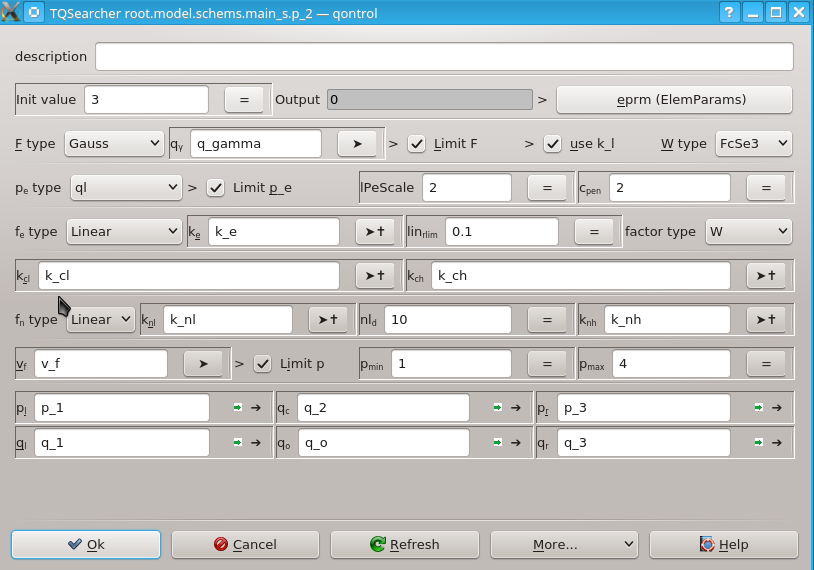
\includegraphics[width=0.7\textwidth]{p/qontrol_tqsearch.png}
  \end{center}
  \caption{Диалоговое окно с элементами интерфейса, автоматически созданными для объекта ``TQSearcher''}
  \label{atu:f:qontrol_qsearch}
\end{figure}

Для обеспечения сигнальной и параметрической связи между элементами
моделируемой системы, созданы классы LinkedObj, InputAbstract,
InputSimple, InputLogic, ParamDouble.
Класс LinkedObj позволяет реализовывать связь между элементами в момент выполнения,
причём с минимальными накладными расходами, на уровне доступа по указателю.
Любой класс, который может быть источником данных, должен быть его открытым наследником.
При этом автоматически учитывается иерархическая структура
и доступ к вложенным элементам.
В качестве структурного элемента, который является приёмником
данных, может выступать наследник InputAbstract.
Объекты типа InputSimple реализуют простую сигнальною связь.
Источником может быть любой элемент схемы, параметр
модели в целом, текущей задачи моделирования, просто константа.
При этом каждый такой вход имеет независимый множитель и смещение,
а также параметры отображения на схеме модели~(рис.~\ref{atu:f:qontrol_link}).


\begin{figure}[htb!]
  \begin{center}
    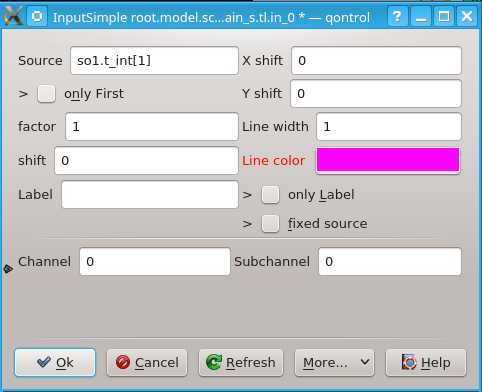
\includegraphics[width=0.5\textwidth]{p/qontrol_link.png}
  \end{center}
  \caption{Диалоговое окно для редактирования элемента типа InputSimple, для определения параметров сигнальной связи между объектами}
  \label{atu:f:qontrol_link}
\end{figure}

Для тех элементов, которые подразумевают наличие переменного количества входов,
например, координатора поиска, важными параметрами входов являются
``channel'' и ``subchannel'', задающие соответственно
номер входного канала и субканала. Для координатора поиска
номер канала задаёт номер соответствующего агента,
а номер субканала - величины $p_e$ и $F$ соответственно.

Некоторые связи представляют собой логические величины,
например, сигналы разрешения работы элемента,
входные сигналы для счётчиков, триггеров и подобных.
Для их обработки создан отдельный класс - InputLogic.
Экземпляры этого класса выполняют те же действия,
что и InputSimple, при этом сигнал приводится
к логическому виду по заданным правилам.
Помимо простого порогового разделения,
реализованы возможности использования триггера Шмидта
и детектора фронтов.

Для реализации параметрических входов используются экземпляры класса ParamDouble.
Отличие их поведения от поведения сигнальных входов заключается в том,
что при изменении значения параметра моделируемым элементом
могут быть предприняты определённые
действия. Если же значением параметра является константа, или же
значение параметра зафиксировано при начале процесса моделирования,
то получение данных происходит только в момент начала моделирования,
что существенно уменьшает вычислительные затраты на численное моделирование.

Базовым классом для всех элементов, которые могут присутствовать
в схеме модели, является TMiso. Он дополняет
возможности, предоставляемые своим базовым классом, LinkedObj,
действиями, выполняемыми непосредственно в процессе
моделирования, перед одним запуском моделирования,
перед группой запусков моделирования, а также после
завершения этих процессов.
Всего у класса TMiso около 50 наследников,
начиная от простых сумматоров, логических элементов,
и заканчивая сложными элементами для реализации
алгоритмов поисковых агентов.

Из всех наследников TMiso следует отметить элемент TSubScheme.
От позволяет в качестве элемента текущей схемы использовать
другую схему. Другая схема может быть как частью модели,
что сейчас используется, так и загружаться из библиотек схем.
Библиотеки схем представляют собой обычные файлы моделей,
которые содержат именованные схемы.

Для получения данных из внешних источников предназначены
два класса: TFileSource и TFileSimple.
Оба позволяют получать данные как из файла, в том числе специального, отображающего
операции ввода-вывода на внешнее устройство или же другой процесс операционной системы.
Первый из них, ценой дополнительных вычислительных затрат позволяет
проводить пере дискретизацию сигнала во временной области.
Второй, за счёт меньших накладных расходов, является более
подходящим при моделировании в реальном масштабе времени.

Объекты типа ``Scheme'' предназначены для объединения элементов модели,
при этом объединены в контейнер схем ``schems'' типа ``ContScheme''.
Гарантируется наличие как минимум одной схемы,
у которой зарезервированное имя ``main\_s''.
Эта схема является основной при моделировании, остальные предназначены для
создания вложенных схем с помощью объектов типа ``TSubScheme''.

Для сбора и обработки данных при моделировании предназначены
объекты типа ``TOutArr'', расположенные в контейнере ``outs'' типа ``ContOut''.
Каждый из них может собирать данный с любого элемента модели,
включая параметры модели, задач моделирования или же других таких же
объектов. При этом можно задать скважность отбора данных,
момент отбора и другие параметры. Также объекты этого пива могут использоваться
как хранилища данных для различных алгоритмов, например
статистического, регрессионного или Фурье анализа. Базовые статистические операции, такие как
вычисления диапазона, среднего, дисперсии происходят автоматически.
Данные могут быть экспортированы, но основное предназначение -
служить основой для построения графиков.

Для построения графиков используются объекты типа TGraph,
расположенные в контейнере ``plots'' типа ``ContOut''.
В каждом из них содержится объект типа ``SchemeData'',
содержащий общую информацию о графике, такую как размер,
цветовая палитра, правила и ограничения при построении осей координат,
легенды и прочее.
Данные, по которым строятся графики, определяются элементами типа
``GraphElem''. Каждый из них задаёт источник данных,
а также определяет, как эти данные будут использоваться:
как данные для осей координат, двумерных или трёхмерных графиков разных типов,
задают цвет или прозрачность.
Одновременно могут быть созданы несколько графиков различных типов,
но с совпадающими осями координат.
Отображением графиков можно управлять как с помощью интерфейса пользователя,
так и с помощью скриптов.

Помимо графиков, на изображении могут быть расположены
метки (PlotLabel) и простейшие графические примитивы (PlotFlippery),
причем координаты и тех и других могут задаваться на основании
любых числовых параметров модели.
Текст меток также может определяться данными модели, при этом
есть возможность задавать формат выводимых данных.
Для вывода специальных математических символов, букв греческого алфавита
используется подмножество математических команд \LaTeX-а.
Помимо отображения на графиках, метки могут использоваться
как часть шаблона имени файла при экспорте изображения,
а также сохраняться в качестве мета информации файла.

Для отображения графиков используется
Mathgl ---
кроссплатформенная библиотека для подготовки высококачественных научных иллюстраций.
Помимо отображения графиков, соответствующие кона предоставляют
набор простых инструментов для анализа~(рис.~\ref{atu:f:qontrol_3d}).


\begin{figure}[htb!]
  \begin{center}
    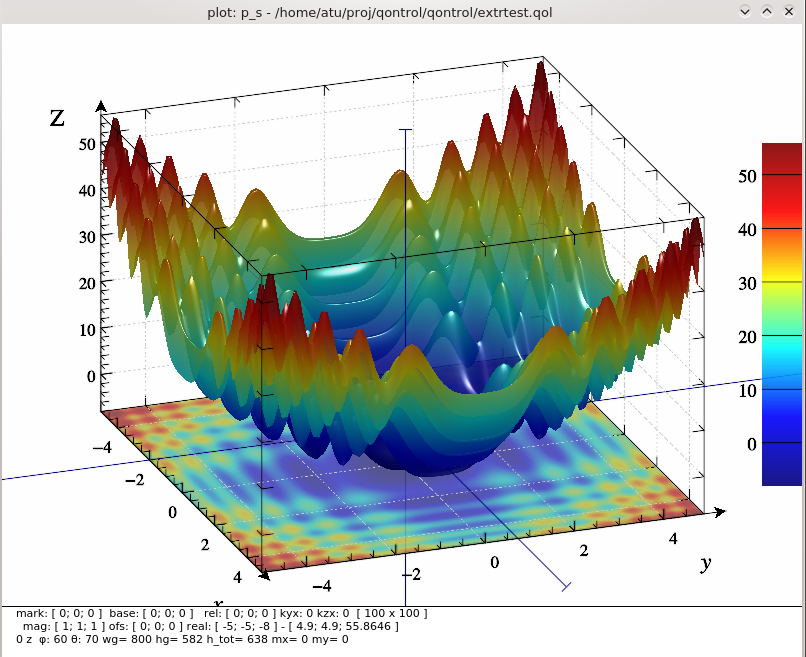
\includegraphics[width=0.7\textwidth]{p/qontrol_3d_a.png}
  \end{center}
  \caption{Окно, предназначенное для отображения графиков в программе ``qontrol''}
  \label{atu:f:qontrol_3d}
\end{figure}

Параметры моделирования (симуляции) задаются объектами типа ``Simulation'',
расположенными в контейнере ``sims'' типа ``ContSimul''.
Всегда существует объект с именем ``sim0'',
определяющим симуляцию по умолчанию.
Параметры этих объектов задают тип моделирования
(простое моделирование, одно и двух параметрическая итерация),
полное время и шаг моделирования,
имена вызываемых функций скриптов на различных стадиях,
а также произвольный набор параметром, типы, имена и значения которых
задаёт пользователь~(рис.~\ref{atu:f:qontrol_simul}).
Модель может содержать произвольное количество стимуляций,
но одновременно выполнятся может только одна.

\begin{figure}[htb!]
  \begin{center}
    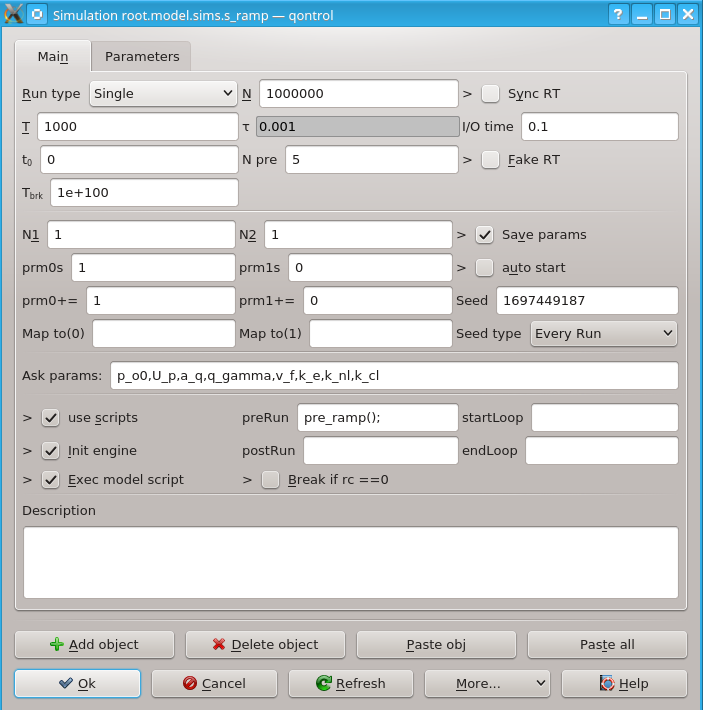
\includegraphics[width=0.7\textwidth]{p/qontrol_task.png}
  \end{center}
  \caption{Диалоговое окно, предназначенное для задания параметров моделирования (Simulation)}
  \label{atu:f:qontrol_simul}
\end{figure}


Центральный объект, объединяющий всю иерархию модели,
называется ``model'' и имеет тип ``TModel''.
Помимо уже упомянутых контейнеров ``schems'', ``outs'', ``sims'', ``schems'',
этот объект содержит свой произвольный набор параметров.
При моделировании, параметры симуляции имеют приоритет
над параметрами модели, что позволяет гибко управлять
наборами параметров при проведении вычислительных экспериментов.

Объект ``model'' также содержит элемент ``script'',
который может содержать используемые в процессе моделирования
скрипты в виде функция на языке JavaScript.
При моделировании все объекты, участвующие
в процессе, импортируются в текущую область видимости
под своими именами~(рис.\ref{atu:f:qontrol_js}).


\begin{figure}[htb!]
  \begin{center}
    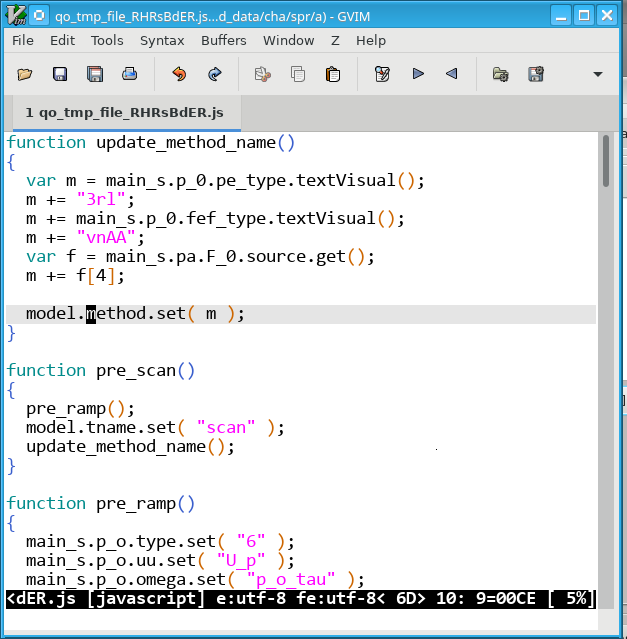
\includegraphics[width=0.6\textwidth]{p/qontrol_js.png}
  \end{center}
  \caption{Пример скриптов программы ``qontrol''}
  \label{atu:f:qontrol_js}
\end{figure}



% }}}2




% }}}1

\section{Пользовательский интерфейс комплекса} %  % {{{1 ----------------------------------------

Пользовательский интерфейс программы ``qontrol'' был создан с помощью
средств, предоставляемых библиотекой Qt.
Используется классический MDI интерфейс,
то есть для каждой модели создаётся отдельное окно,
отображающее структуру модели, и позволяющее ей изменять~(рис.~\ref{atu:f:qontrol_all}).
Помимо основного окна, для каждой модели может быть открыть
произвольное число окон отображения графиков и редактирования суб схем.


\begin{figure}[htb!]
  \begin{center}
    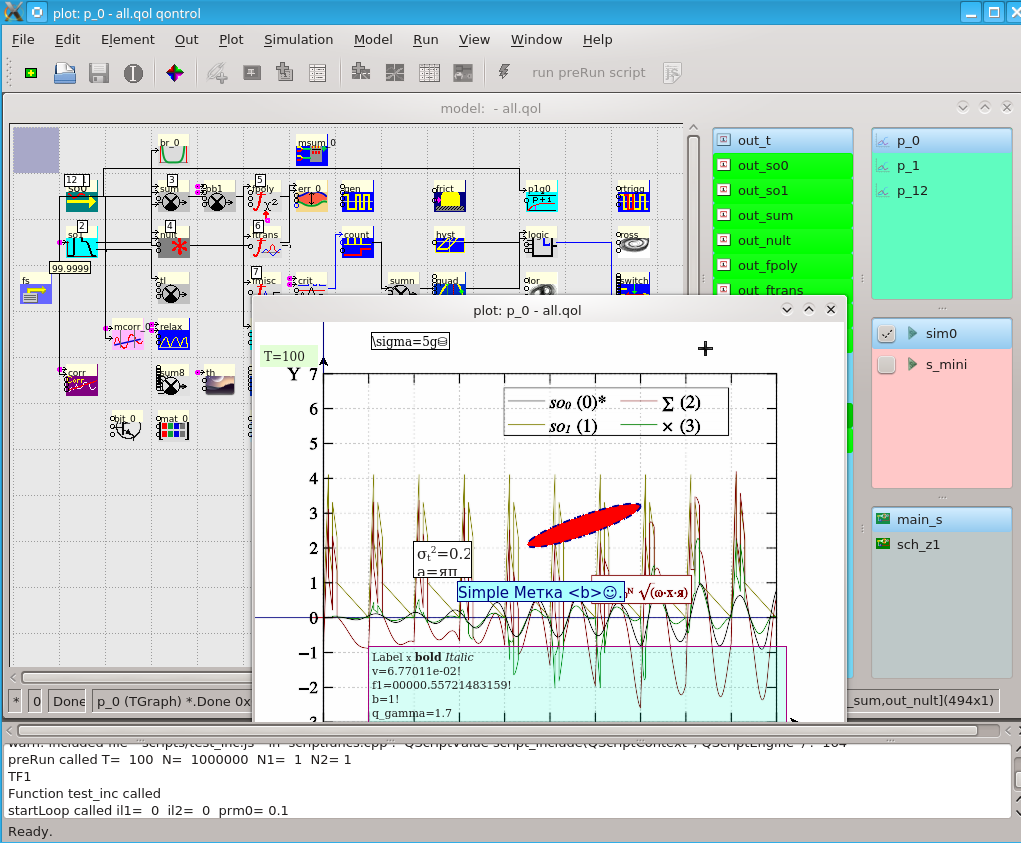
\includegraphics[width=0.96\textwidth]{p/qontrol_all.png}
  \end{center}
  \caption{Общий вид интерфейса пользователя программы ``qontrol''}
  \label{atu:f:qontrol_all}
\end{figure}

Центральную часть окна занимает редактор основной схемы моделей.
После моделирования там также могут быть отображены
произвольные данные, связанные с элементами модели.

В правой части окна расположены списки объектов сбора данных,
графиков, параметров моделирования и схем.
Нижнюю часть окна занимает область вывода,
в которую поступают сообщения об ошибках, замечаниях,
а также стандартный вывод скриптов.


Файлы моделей сохраняются в
XML формате с суффиксом ``.qol'', что даёт возможность их редактировать за пределами программы
как с помощью обычных текстовых редакторов, так и с использованием
специальных средств для обработки структурированных XML документов.


Программа может быть запущена и без графического интерфейса.
При этом обязательно указание в командной строке
имени модели. Дополнительно указывается имя симуляции,
задаются параметры моделирования, и, при необходимости,
указания о том, куда и как сохранять полученные данные и
созданные графики.

% }}}1


\section{Выводы по разделу \thechapter} %  % {{{1 ---------------------------------------------

Создана программная среда ``qontrol'', предназначенная для моделирования
нелинейных динамических систем, обладает набором качеств,
которые существенно упрощают процесс моделирования,
создания новых систем идентификации и управления.
К характеристикам программы следует отнести:

\begin{itemize}

  \item
    Универсальность, позволяющая создавать модели сложных динамических систем,
    с возможностью комбинирования и группировки элементов системы.

  \item
    Развитые средства обработки и представления данных.

  \item
    Удобный интерфейс пользователя.

  \item
    Высокая скорость моделирования.

  \item
    Возможность запускать программу в консольном режиме, без графического интерфейса
    для проведения моделирования в пакетном режиме.

  \item
    Автоматическое построение интерфейса пользователя на основе
    данных, представляемых моделируемым элементом.

  \item
    Возможность реализации сложных задач моделирования, которые не вписываются
    в набор базовых действий, за счёт применения встроенного языка программирования,
    основанного на JavaScript, и возможностью доступа к функциям программной среды.

  \item
    Широкие возможности по отображение информации в графическом виде.

  \item
    Возможность взаимодействия с другими программными и аппаратно-программными
    комплексами.


  \item
    Открытый исходный код, что даёт возможность как применять элементы созданной
    программы в своих разработках, так и дополнять программу своими элементами.


  \item
    Open-source лицензия и свободное распространение,
    что позволяет без существенных затрат использовать программную среду
    при проведении исследований и в учебном процессе.

\end{itemize}


% }}}1


% vim: fdm=marker ft=tex
